\documentclass[12pt]{article}
\usepackage[romanian]{babel}
\usepackage{graphicx}
\usepackage{caption}
\usepackage{booktabs}
\usepackage{amsmath}
\usepackage[a4paper, margin=1in]{geometry}
\usepackage{tikz}
\usepackage{hyperref}

\title{\vspace{-4cm} 
       \Huge Securitatea în Rețelele de Calculatoare}
\author{\Large Farcaș Alexandru Alin}
\date{\Large 23 Ianuarie, 2024}

\begin{document}

\begin{titlepage}
    \centering 
    \vspace*{1cm} 
    {\Huge\bfseries Securitatea în Rețelele de Calculatoare \par}
    \vspace{1.5cm}
    {\Large Farcaș Alexandru Alin\par}
    \vspace{2cm}
    
    \rule{\textwidth}{0.4pt}  % Linie orizontală
    \vspace{0.5cm}
    
    {\Large\textit{Prof. coordonator:} \par}
    \vspace{0.25cm}
    {\Large Palcu Adrian \par}
    {\Large Gavrilă Tania \par}
    
    \vspace{2cm}
    {\Large 23 Ianuarie, 2024\par}
\end{titlepage}

\newpage
\tableofcontents
\newpage


\section{Introducere}
În era digitală contemporană, securitatea rețelelor de calculatoare a devenit un pilon fundamental pentru protejarea integrității și confidențialității datelor în mediul online. Această secțiune introduce conceptele cheie ale securității cibernetice, subliniind importanța lor în lumea tehnologică accelerată de astăzi.

Securitatea rețelelor de calculatoare nu este doar o preocupare tehnică, ci una care afectează fiecare aspect al societății moderne. De la tranzacțiile financiare până la comunicările personale și de afaceri, aproape fiecare facțiune a vieții noastre cotidiene este interconectată printr-o rețea vastă și complexă de calculatoare și servere. Prin urmare, vulnerabilitățile din aceste sisteme nu doar că amenință datele individuale, ci pot avea și implicații mai largi asupra securității naționale, economice și sociale.

Pe măsură ce tehnologia avansează, și natura amenințărilor evoluează. Atacurile cibernetice au devenit mai sofisticate, punându-i pe specialiștii în securitate în fața unor provocări fără precedent. Acest lucru este accentuat de creșterea IoT (Internet of Things), unde milioane de dispozitive conectate la internet devin ținte potențiale pentru actorii rău intenționați. Astfel, securitatea rețelelor nu se mai limitează doar la computere și servere, ci se extinde la o gamă largă de dispozitive inteligente, de la smartphone-uri la electrocasnice conectate.

În acest context, proiectul nostru se propune să exploreze diversele aspecte ale securității în rețelele de calculatoare, analizând strategiile și tehnologiile actuale utilizate pentru a contracara amenințările cibernetice. De asemenea, vom arunca o privire asupra viitorului securității cibernetice, anticipând evoluțiile tehnologice și adaptându-ne la schimbările continue din peisajul amenințărilor.

Prin urmare, această introducere setează scena pentru o explorare detaliată și cuprinzătoare a securității în rețelele de calculatoare, un domeniu care devine din ce în ce mai relevant și vital în lumea noastră interconectată.


\newpage
\section{Fundamente Teoretice}
Un aspect central al securității rețelelor îl reprezintă înțelegerea și aplicarea protocoalelor de rețea. Protocoalele, cum ar fi TCP/IP (Transmission Control Protocol/Internet Protocol), sunt esențiale pentru funcționarea internetului și a rețelelor. Acestea reglementează modul în care datele sunt trimise și primite peste rețea, asigurându-se că informațiile ajung la destinație într-o manieră ordonată și fiabilă. De asemenea, protocoalele de securitate precum HTTPS (Hypertext Transfer Protocol Secure), SSL/TLS (Secure Sockets Layer/Transport Layer Security) și VPN-urile (Virtual Private Networks) sunt vitale pentru asigurarea unui schimb sigur de date.

O altă componentă esențială este criptografia, care este arta și știința de a proteja informațiile prin transformarea lor într-un format indecidabil, numit criptare, astfel încât doar cei care dețin o cheie secretă pot accesa informațiile originale, printr-un proces numit decriptare. De la criptografia simetrică, unde aceeași cheie este folosită atât pentru criptare cât și pentru decriptare, la criptografia asimetrică, care folosește o pereche de chei publică și privată, aceste tehnici sunt fundamentale pentru protejarea comunicațiilor și a datelor.

În plus, acest capitol examinează și alte tehnologii și practici esențiale în securitatea rețelelor, cum ar fi firewall-urile, sistemele de detectare și prevenire a intruziunilor (IDS/IPS), și autentificarea multi-factor. Firewall-urile servesc ca o primă linie de apărare, controlând traficul de rețea pentru a preveni accesul neautorizat. IDS/IPS monitorizează rețeaua pentru activități suspecte și încearcă să prevină sau să minimizeze atacurile. Autentificarea multi-factor adaugă un nivel suplimentar de securitate, solicitând utilizatorilor să furnizeze două sau mai multe dovezi de identitate înainte de a accesa sistemele.

\newpage
\subsection{Formule Matematice}
Securitatea în rețelele de calculatoare se bazează adesea pe principii matematice complexe, în special în domeniul criptografiei. Această subsecțiune prezintă câteva dintre formulele fundamentale utilizate în criptografia simetrică și asimetrică.

\subsubsection{Criptografia Simetrică}
În criptografia simetrică, aceeași cheie (\( k \)) este utilizată atât pentru criptare cât și pentru decriptare. Funcția de criptare poate fi reprezentată ca:
\begin{equation}
    E_k(M) = C
\end{equation}
unde \( E_k \) este funcția de criptare cu cheia \( k \), \( M \) este mesajul clar, și \( C \) este mesajul criptat. Invers, funcția de decriptare este:
\begin{equation}
    D_k(C) = M 
\end{equation}
unde \( D_k \) este funcția de decriptare.

\subsubsection{Criptografia Asimetrică}
Criptografia asimetrică folosește o pereche de chei: o cheie publică (\( k_{pub} \)) și o cheie privată (\( k_{priv} \)). Criptarea și decriptarea se realizează folosind aceste chei diferite. Formulele sunt:
\begin{align}
    E_{k_{pub}}(M) &= C \\
    D_{k_{priv}}(C) &= M
\end{align}
unde \( E_{k_{pub}} \) reprezintă criptarea cu cheia publică, iar \( D_{k_{priv}} \) reprezintă decriptarea cu cheia privată.

\newpage
\section{Studiu de Caz / Analiză}
În această secțiune, analizăm un atac cibernetic semnificativ care a avut loc recent, evidențiind vulnerabilitățile exploatate și măsurile de apărare implementate. Acest studiu de caz oferă perspective importante asupra realităților securității cibernetice în practică și ilustrează complexitatea apărării împotriva amenințărilor moderne.

\subsection{Descrierea Atacului}
Descrieți aici detaliile atacului, inclusiv momentul când a avut loc, natura vulnerabilității exploatate, tipul de atac (de exemplu, ransomware, phishing, DDoS) și impactul său asupra organizației țintă. Discutați despre modul în care atacul a fost detectat și răspunsul inițial.

\subsection{Analiza Tehnică}
Oferiți o analiză tehnică a atacului, explicând cum atacatorii au reușit să penetreze sistemele de securitate. Includeți detalii despre metodele și tehnologiile folosite atât de atacatori, cât și de apărători. Această parte poate include un fragment de cod sursă, exemplificând un tipar de cod vulnerabil sau o metodă de detectare a atacurilor.

\begin{verbatim}
// Exemplu de cod vulnerabil sau metodă de detectare
#include <stdio.h>
int main() {
    // Detalii tehnice ale codului
    return 0;
}
\end{verbatim}

\subsection{Grafice și Tabele}

\begin{figure}[h]
\centering
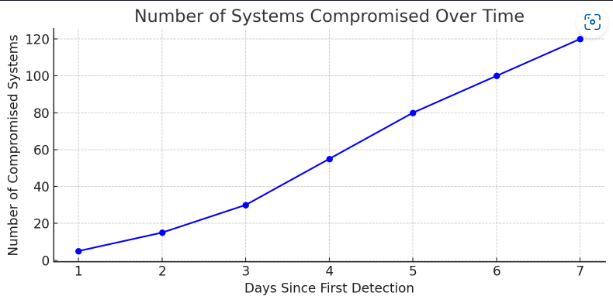
\includegraphics[width=0.8\textwidth]{poze/grafic detectie.png}
\caption{Grafic ilustrativ pentru atacul cibernetic analizat}
\end{figure}

\subsection{Concluzii Studiu de Caz}
Discutați implicațiile atacului și lecțiile învățate. Analizați eficacitatea măsurilor de răspuns și cum acest studiu de caz poate informa strategiile de securitate viitoare. Este important să reflectăm asupra modurilor prin care organizațiile pot îmbunătăți continuu practicile de securitate pentru a rămâne înaintea atacatorilor cibernetici.

\subsection{Cod Sursă}
În această subsecțiune, prezentăm un exemplu de pseudocod care ilustrează cum un sistem de detectare a intruziunilor ar putea identifica un atac cibernetic, bazat pe un model de comportament neobișnuit sau semnături specifice.

\begin{verbatim}
// Pseudocod pentru un simplu sistem de detectare a intruziunilor
#include <stdio.h>
int detectCyberAttack() {
    // Pseudocod pentru detectarea unui model de trafic neobișnuit
    if (detectUnusualTrafficPatterns()) {
        printf("Atac cibernetic detectat!\n");
        return 1; // Indică detectarea unui atac
    } else {
        printf("Traficul de rețea este normal.\n");
        return 0; // Niciun atac detectat
    }
}

int main() {
    int attackDetected = detectCyberAttack();
    if (attackDetected) {
        // Implementați măsuri de răspuns la incident
    }
    return 0;
}
\end{verbatim}


\newpage
\section{Rezultate și Discuții}
Această secțiune discută rezultatele analizei studiului de caz, evaluând eficacitatea răspunsului la atac și lecțiile învățate. Se vor examina strategiile implementate și impactul lor asupra organizației.

\subsection{Evaluarea Răspunsului la Atac}
Discutăm eficacitatea răspunsului organizației, inclusiv detectarea rapidă a atacului și neutralizarea acestuia.

\subsection{Analiza Impactului Atacului}
Analizăm impactul atacului asupra organizației, incluzând pierderile de date și financiare.

\subsection{Grafice și Tabele cu Analiza Datelor}
\begin{figure}[h]
\centering
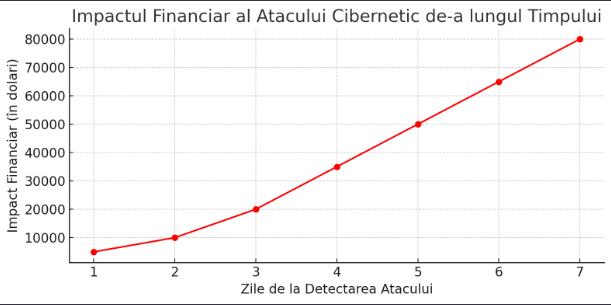
\includegraphics[width=0.6\textwidth]{poze/grafic cap4.png}
\caption{Grafic cu Analiza Impactului Atacului Cibernetic}
\end{figure}

\subsection{Lecții Învățate și Îmbunătățiri Propuse}
Detaliem lecțiile învățate și propunem îmbunătățiri pentru strategiile de securitate.

\subsection{Rezumatul Răspunsurilor la Atac}
\begin{table}[h]
\centering
\begin{tabular}{@{}lll@{}}
\toprule
Acțiune de Răspuns & Eficiența & Îmbunătățiri Propuse \\ \midrule
Detectare Rapidă & Medie & Îmbunătățirea sistemelor \\
Neutralizarea Atacului & Înaltă & Revizuirea procedurilor \\
Comunicarea cu Părțile & Scăzută & Plan de comunicare \\
Analiza Post-Atac & Înaltă & Analiză periodică \\
Formarea Angajaților & Medie & Programe de conștientizare \\ \bottomrule
\end{tabular}
\caption{Rezumatul Răspunsurilor la Atacul Cibernetic}
\end{table}


\newpage
\section{Concluzii}
Acest proiect a explorat în profunzime securitatea în rețelele de calculatoare, un domeniu esențial și în continuă evoluție în era digitală. Am demonstrat cum vulnerabilitățile din rețelele de calculatoare pot avea implicații extinse, afectând nu doar datele individuale, ci și securitatea națională și economică.

Principalele puncte subliniate în acest proiect includ importanța înțelegerii protocoalelor de rețea și a criptografiei în protecția datelor. Studiul de caz analizat a ilustrat complexitatea și sofisticarea atacurilor cibernetice actuale, precum și necesitatea unor răspunsuri rapide și eficiente. Am văzut că măsurile de securitate nu sunt doar despre tehnologie, ci și despre oameni; formarea și conștientizarea angajaților sunt vitale.

Am învățat că, în fața amenințărilor cibernetice, nu există o soluție unică sau definitivă. Securitatea rețelelor necesită o abordare adaptabilă și dinamică, capabilă să răspundă rapid la noile provocări. Este esențială o actualizare continuă a cunoștințelor și a tehnologiilor de securitate, precum și o colaborare strânsă între diferitele sectoare pentru a combate eficient atacurile cibernetice.

În concluzie, securitatea rețelelor de calculatoare este un aspect fundamental al societății noastre interconectate și va continua să fie o prioritate majoră într-o lume digitală în permanentă schimbare. Prin acest proiect, am subliniat necesitatea unei abordări holistice și bine informate în domeniul securității cibernetice, un domeniu care necesită atenție constantă și adaptabilitate.

\newpage
\addcontentsline{toc}{section}{Bibliografie}

\begin{thebibliography}{Bibliografie}

\bibitem{ciscosecurity}
Cisco Networking Academy,
\textit{Introducere în Securitatea Rețelelor, \url{https://www.netacad.com/courses/cybersecurity/introduction-network-security}},
2023.

\bibitem{microsoftsecurity}
Microsoft Docs,
\textit{Înțelegerea Fundamentelor Securității Cibernetice, \url{https://docs.microsoft.com/en-us/learn/paths/understand-cybersecurity-fundamentals/}},
2023.

\bibitem{rsacrypto}
RSA Laboratories,
\textit{Criptografia RSA Astăzi, \url{https://www.rsa.com/en-us/research-and-thought-leadership/cryptography}},
2023.

\bibitem{nistcrypto}
National Institute of Standards and Technology,
\textit{Standarde și Ghiduri Criptografice, \url{https://csrc.nist.gov/projects/cryptographic-standards-and-guidelines}},
2023.

\bibitem{kasperskycyber}
Kaspersky,
\textit{Anatomia unui Atac Cibernetic, \url{https://www.kaspersky.com/resource-center/preemptive-safety/anatomy-of-a-cyber-attack}},
2023.

\bibitem{symantecreport}
Symantec,
\textit{Raportul Privind Amenințările de Securitate pe Internet, \url{https://www.broadcom.com/company/newsroom/press-releases}},
2023.

\bibitem{csoonline}
CSO Online,
\textit{Cele Mai Mari Breșe de Date ale Secolului 21, \url{https://www.csoonline.com/article/2130877/the-biggest-data-breaches-of-the-21st-century.html}},
2023.

\bibitem{infosecmagazine}
Infosecurity Magazine,
\textit{Înțelegerea Impactului Atacurilor Cibernetice asupra Afacerilor, \url{https://www.infosecurity-magazine.com/}},
2023.

\bibitem{hbrsecurity}
Harvard Business Review,
\textit{Factorul Uman în Securitatea Cibernetică: Lecții de la Pentagon, \url{https://hbr.org/2023/01/cybersecuritys-human-factor-lessons-from-the-pentagon}},
2023.

\end{thebibliography}
\end{document}


